\documentclass[12pt]{article}


\usepackage[utf8]{inputenc} % allow utf-8 input
\usepackage[T1]{fontenc}    % use 8-bit T1 fonts
\usepackage{kpfonts}

\usepackage{hyperref}       % hyperlinks
\usepackage{url}            % simple URL typesetting
\usepackage{booktabs}       % professional-quality tables
\usepackage{amsfonts}       % blackboard math symbols
\usepackage{nicefrac}       % compact symbols for 1/2, etc.
\usepackage{microtype}
\usepackage{amsmath}      % microtypography
\usepackage{bm}
\usepackage{graphicx}
\usepackage{verbatim}
\usepackage{wrapfig}
\usepackage[font=small]{caption}
\usepackage{enumitem}
%\usepackage{amsmath}
%\usepackage{floatrow}

\usepackage[legalpaper, margin=1in]{geometry}

\usepackage{setspace}
\setstretch{1.2}

%\addtolength{\belowcaptionskip}{-20pt}

\title{Project progress report}

\begin{document}

\maketitle


\section{Introduction}

Traditional approaches for RNA secondary structure prediction uses either dynamic programming
with experimentally measured hard-coded free energy terms,
or formulate the folding problem as syntax parsing under some stochastic context free grammar,
and tries to learn the parameters from training dataset.
Both types of approaches are very similar in their nature, in the sense that
they all rely on recursion at the base-pair level.
These methods predict structures that satisfy all hard constraints since the
underlying recursion is designed to only generate valid sequence and structures.
In addition, there is typically an efficient way to sample sub optimal structure by
stochastic trace back.
On the other hand, the expressiveness of these models is heavily restricted by the underlying
recursion, and strong assumptions have to be made for the recursion to be tractable
(for example, the nested assumption makes predicting pseudoknot an impossible task).

Recently there have been several work that uses neural network to tackle the structure prediction
problem end-to-end. These models benefit from the fact that they are highly expressive and can be trained on lot of data,
but most of the work ignore the hard constraint completely.
One interesting work (SPOT-RNA) proposed to add a fixed layer RNN representing an unrolled
constrained optimization, to convert the neural network output to one that satisfy the hard constraints.
One potential is that there is no convergence guarantee, and even if it converges there's guarantee the output satisfies the constraints,
since the original discrete optimization problem need to be relaxed in order to run through the optimization RNN.


In this work we aim at developing a model that makes use of the expressiveness of deep neural network
while respecting all the hard constraints. This report covers the following topics:

\begin{itemize}
    \item review the commonly used data representation for RNA secondary structure
    \item propose an alternative way to represent the structure, using the idea of local structural components
    \item describe a 2-stage model under the alternative parametrization,
which satisfies the hard constraints by design
    \item present results on stage 1 model
    \item discussion of ideas for stage2 and future improvement
\end{itemize}


\subsection{Problem formulation}

Given an RNA sequence of length $L$, we are interested in its secondary structure(s) (most likely single structure, or a distribution of structures).
%There are three common ways to represent a specific RNA secondary structure:
To represent a specific secondary structure, there are three commonly used conventions:
(1) undirected graph, where each node is a base in the sequence, and each edge represents base pairing.
(2) upper triangular matrix (excluding the diagonal)
of size $L \times L$ with binary values, where a value of $1$ at $(i, j)$ represents
base pairing between sequence position $i$ and $j$, and $0$ represents no base paring.
(3) dot-bracket notation of length $L$ where unpaired bases are denoted as dots,
    and paired bases are represented as left and right brackets.
%When pseudoknot is present, different styles of bracket needs to be used to represent nested structures.
We'll be using the \textit{upper triangular matrix} representation throughout this report.


\begin{figure}[h]
    \centering
    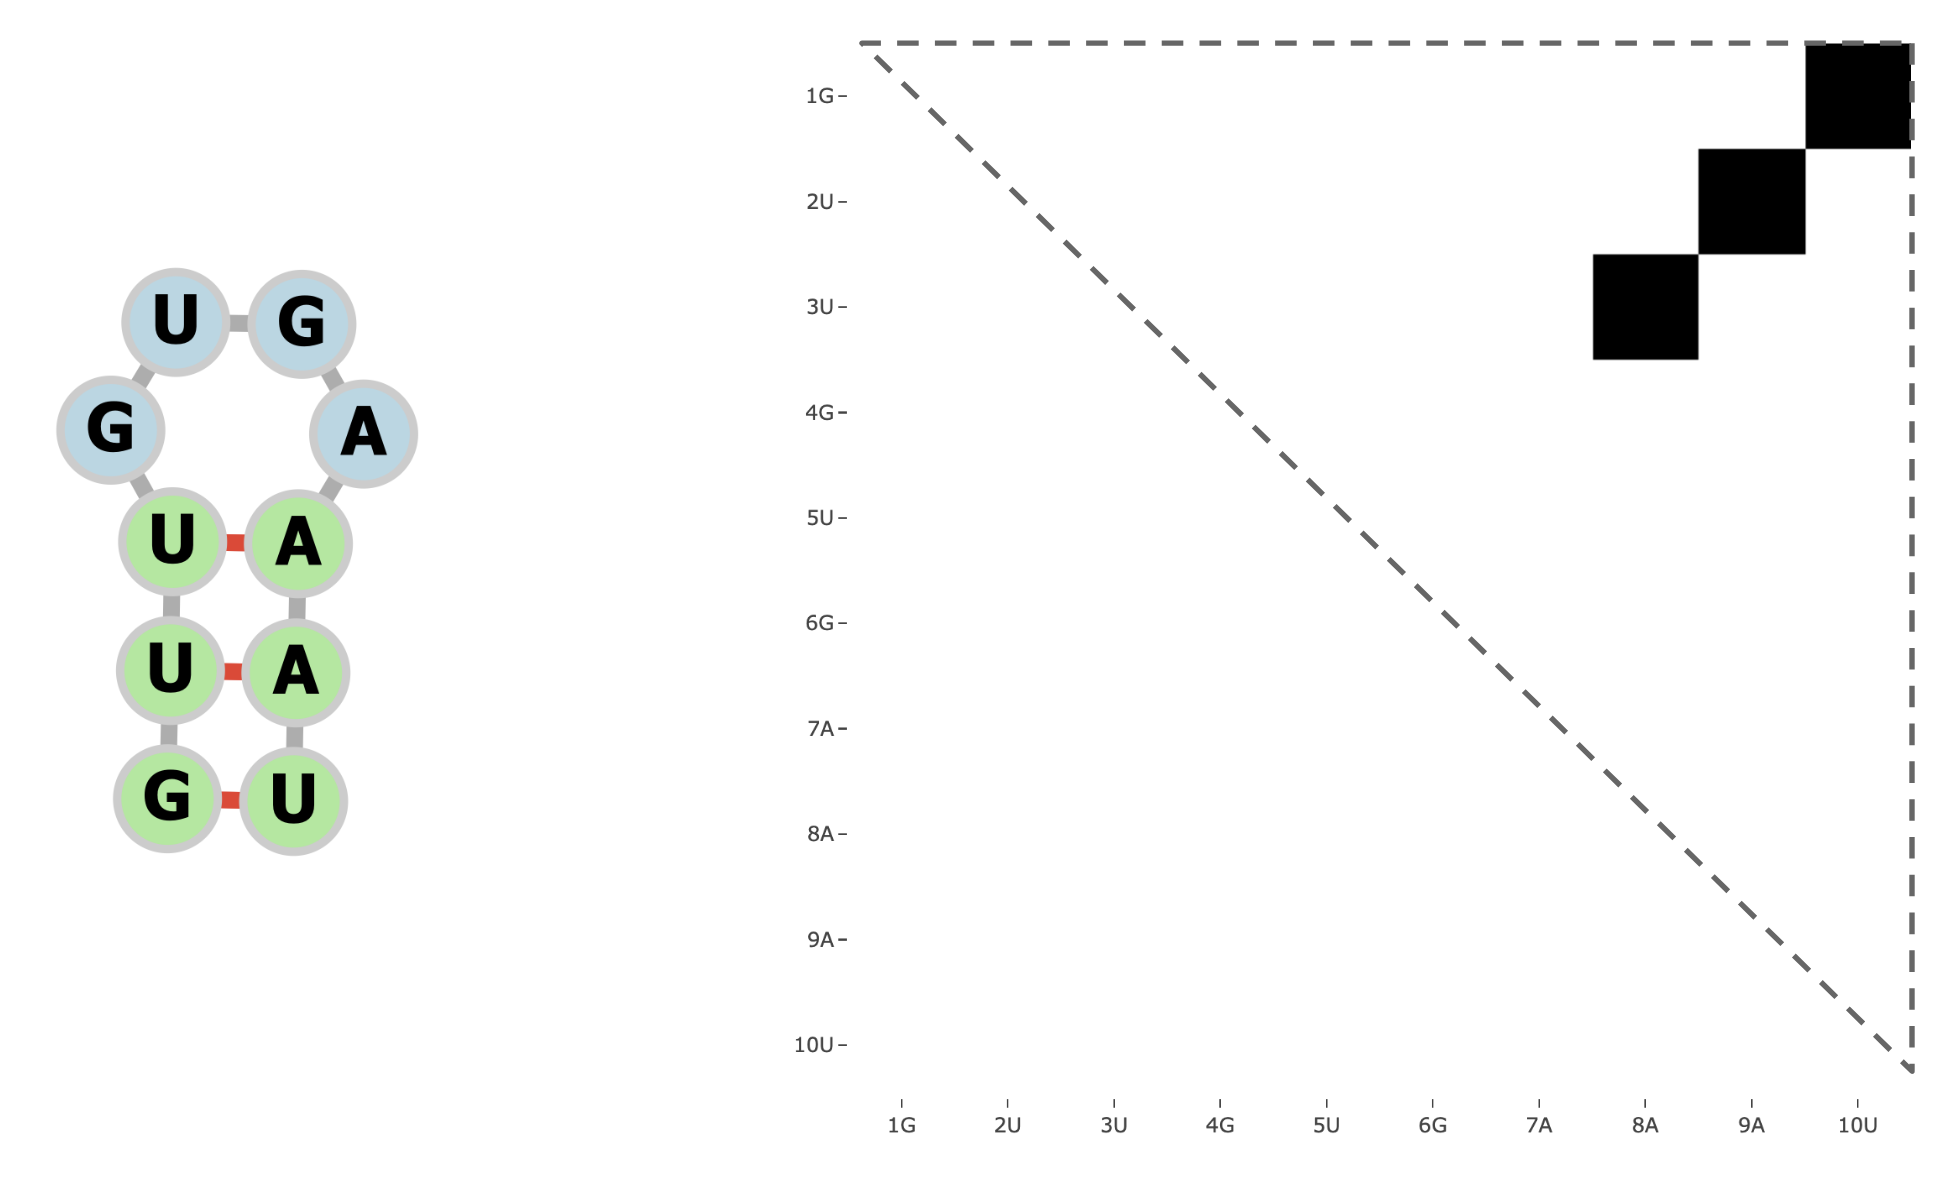
\includegraphics[width=0.8\textwidth]{plot/rna_ss_binary_mat.png}
    \caption{TODO}
    \label{fig:rna_ss_binary_mat}
    \centering
\end{figure}

As an example, for a short RNA sequence GUUGUGAAAU, one possible structure it can take on
consists of a stem and a loop, as seen in Fig \ref{fig:rna_ss_binary_mat} on the left, represented by an undirected graph.
Such structure can also be represented by a $10 \times 10$ upper triangular matrix with all $0$'s,
except for positions
%$y_{1, 10}, y_{2, 9}$ and $y_{3, 8}$,
$(1, 10), (2, 9)$ and $(3, 8)$,
all being $1$, as shown in Fig \ref{fig:rna_ss_binary_mat} on the right.
This contiguous stretch of $1$'s along the diagonal corresponds to the stem formed by the three base pairs: G-U, U-A and U-A.


\section{Structural components}


Just as sequence motif is defined in the linear sequence space,
a similar notion of 'structural motif' also exists.
A commonly adopted way is to break down structure into the following components:

\begin{itemize}
    \item hairpin loop: todo
    \item stem: todo
    \item internal loop: todo
    \item bulge: todo
    \item external loop: todo
    \item multibranch loop: todo
    \item pseudoknot: todo
\end{itemize}

Such structural motifs can be easily identified on the graph representation of a structure,
as shown in Fig \ref{fig:structural_motif_graph}, where we only annotated one instance for
each structural motif class for clarity.
(todo add a minimal example for pseudoknot)

\begin{figure}[h]
    \centering
    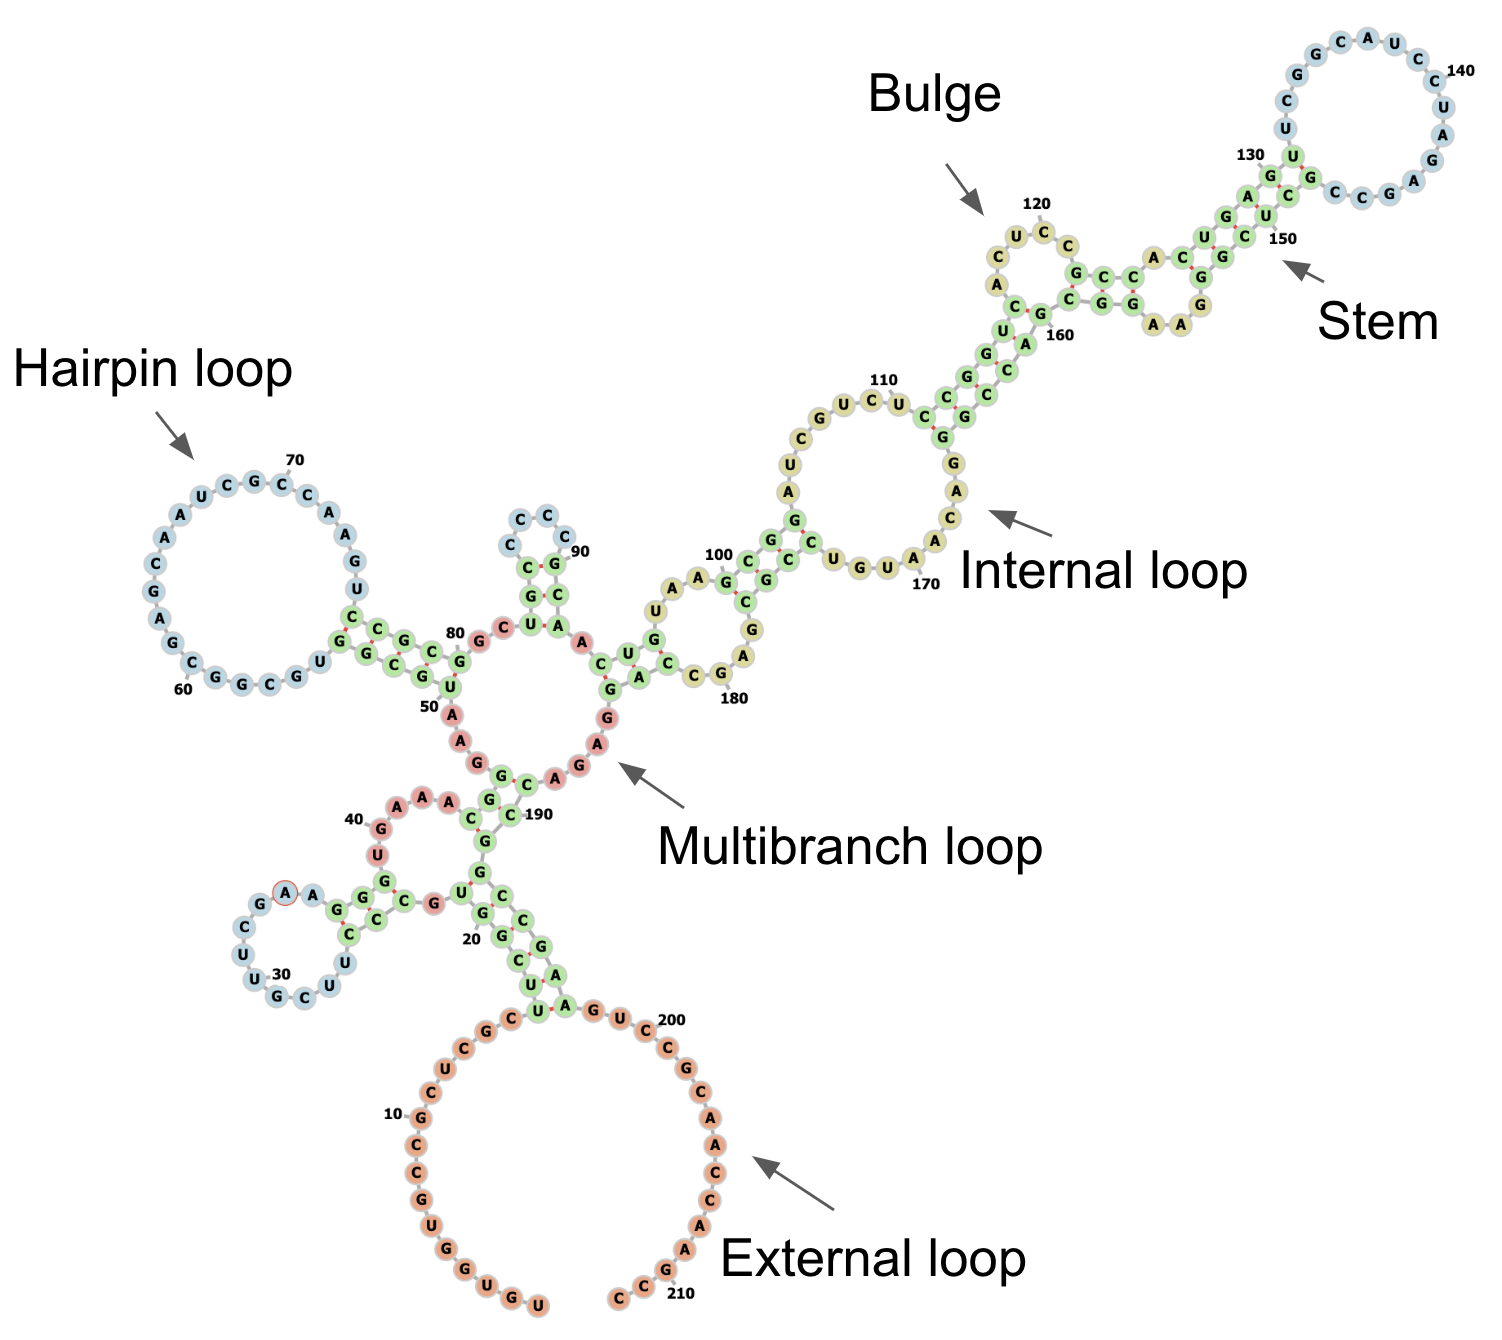
\includegraphics[width=0.8\textwidth]{plot/structural_motif_graph.png}
    \caption{TODO}
    \label{fig:structural_motif_graph}
    \centering
\end{figure}


In this work, we distinguish structural motifs that are 'local' and 'non-local',
where local-ness is defined w.r.t. the 2D matrix representation of the structure.
The importance of such distinction will become clear in Section (todo).
To illustrate this idea, we plot the 2D matrix representation of the above structure
in Fig \ref{fig:structural_motif_2d_matrix}(a),
where majority of the pixels are in *navy* (unpaired positions),
and a few pixels in *yellow* (paired positions).
For each type of structural motif, if it can be fully represented by the interaction between
two (contiguous) substrings of the original sequence, it is considered a 'local' structure,
and can be fully identified by a bounding box on 2D matrix.
Note that interaction does not necessarily mean the substrings bind to each other.
On the other hand, certain structure motifs can only be represented by interaction between
three or more (contiguous) substrings of the original sequence,which we refer to as non-local structures.

\begin{figure}[h]
    \centering
    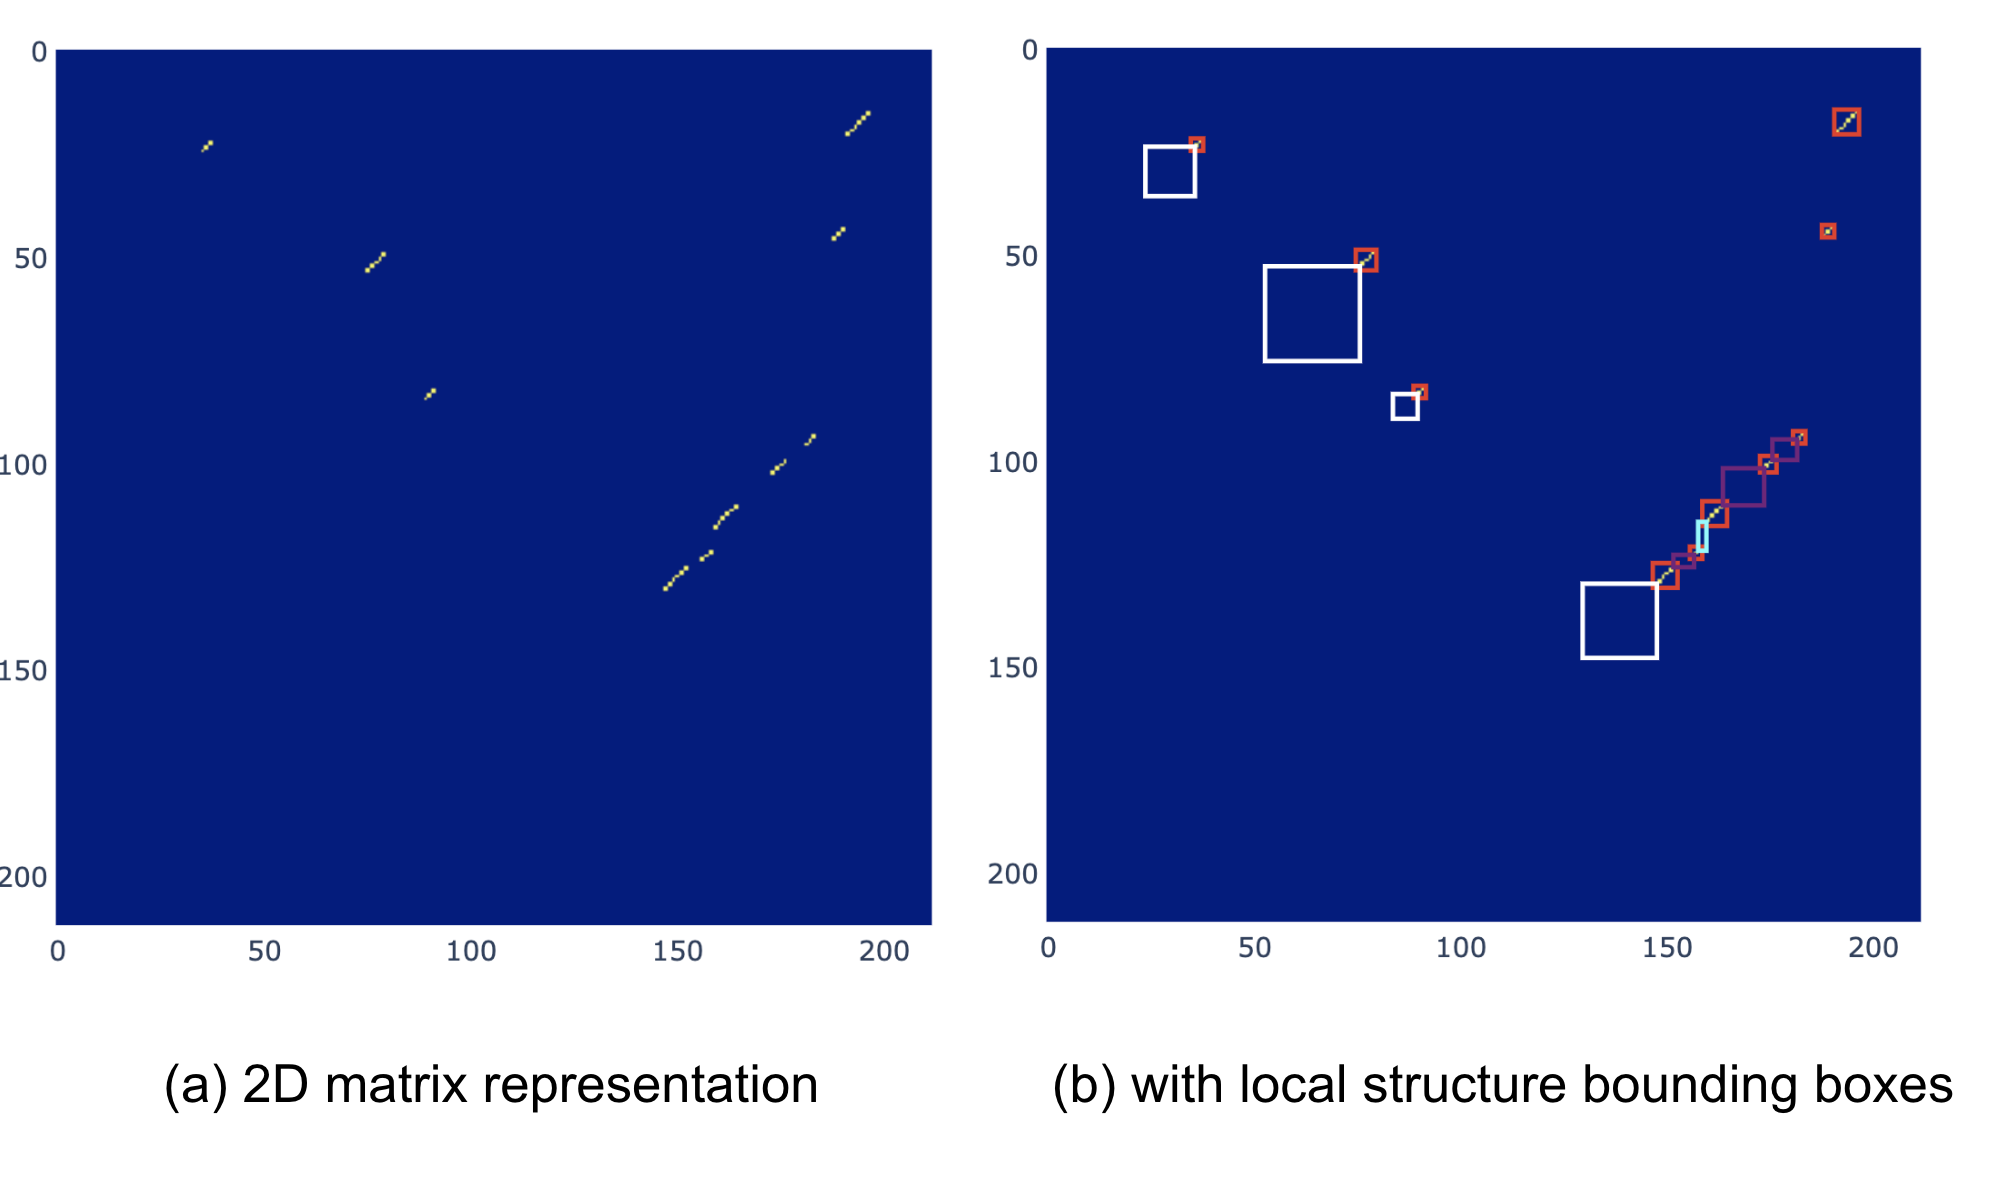
\includegraphics[width=\textwidth]{plot/structural_motif_2d_matrix.png}
    \caption{TODO}
    \label{fig:structural_motif_2d_matrix}
    \centering
\end{figure}


\subsection{Local structures}


Using the above definition, we drew all the local structure bounding boxes
in Fig \ref{fig:structural_motif_2d_matrix}(b).


\begin{figure}[h]
    \centering
    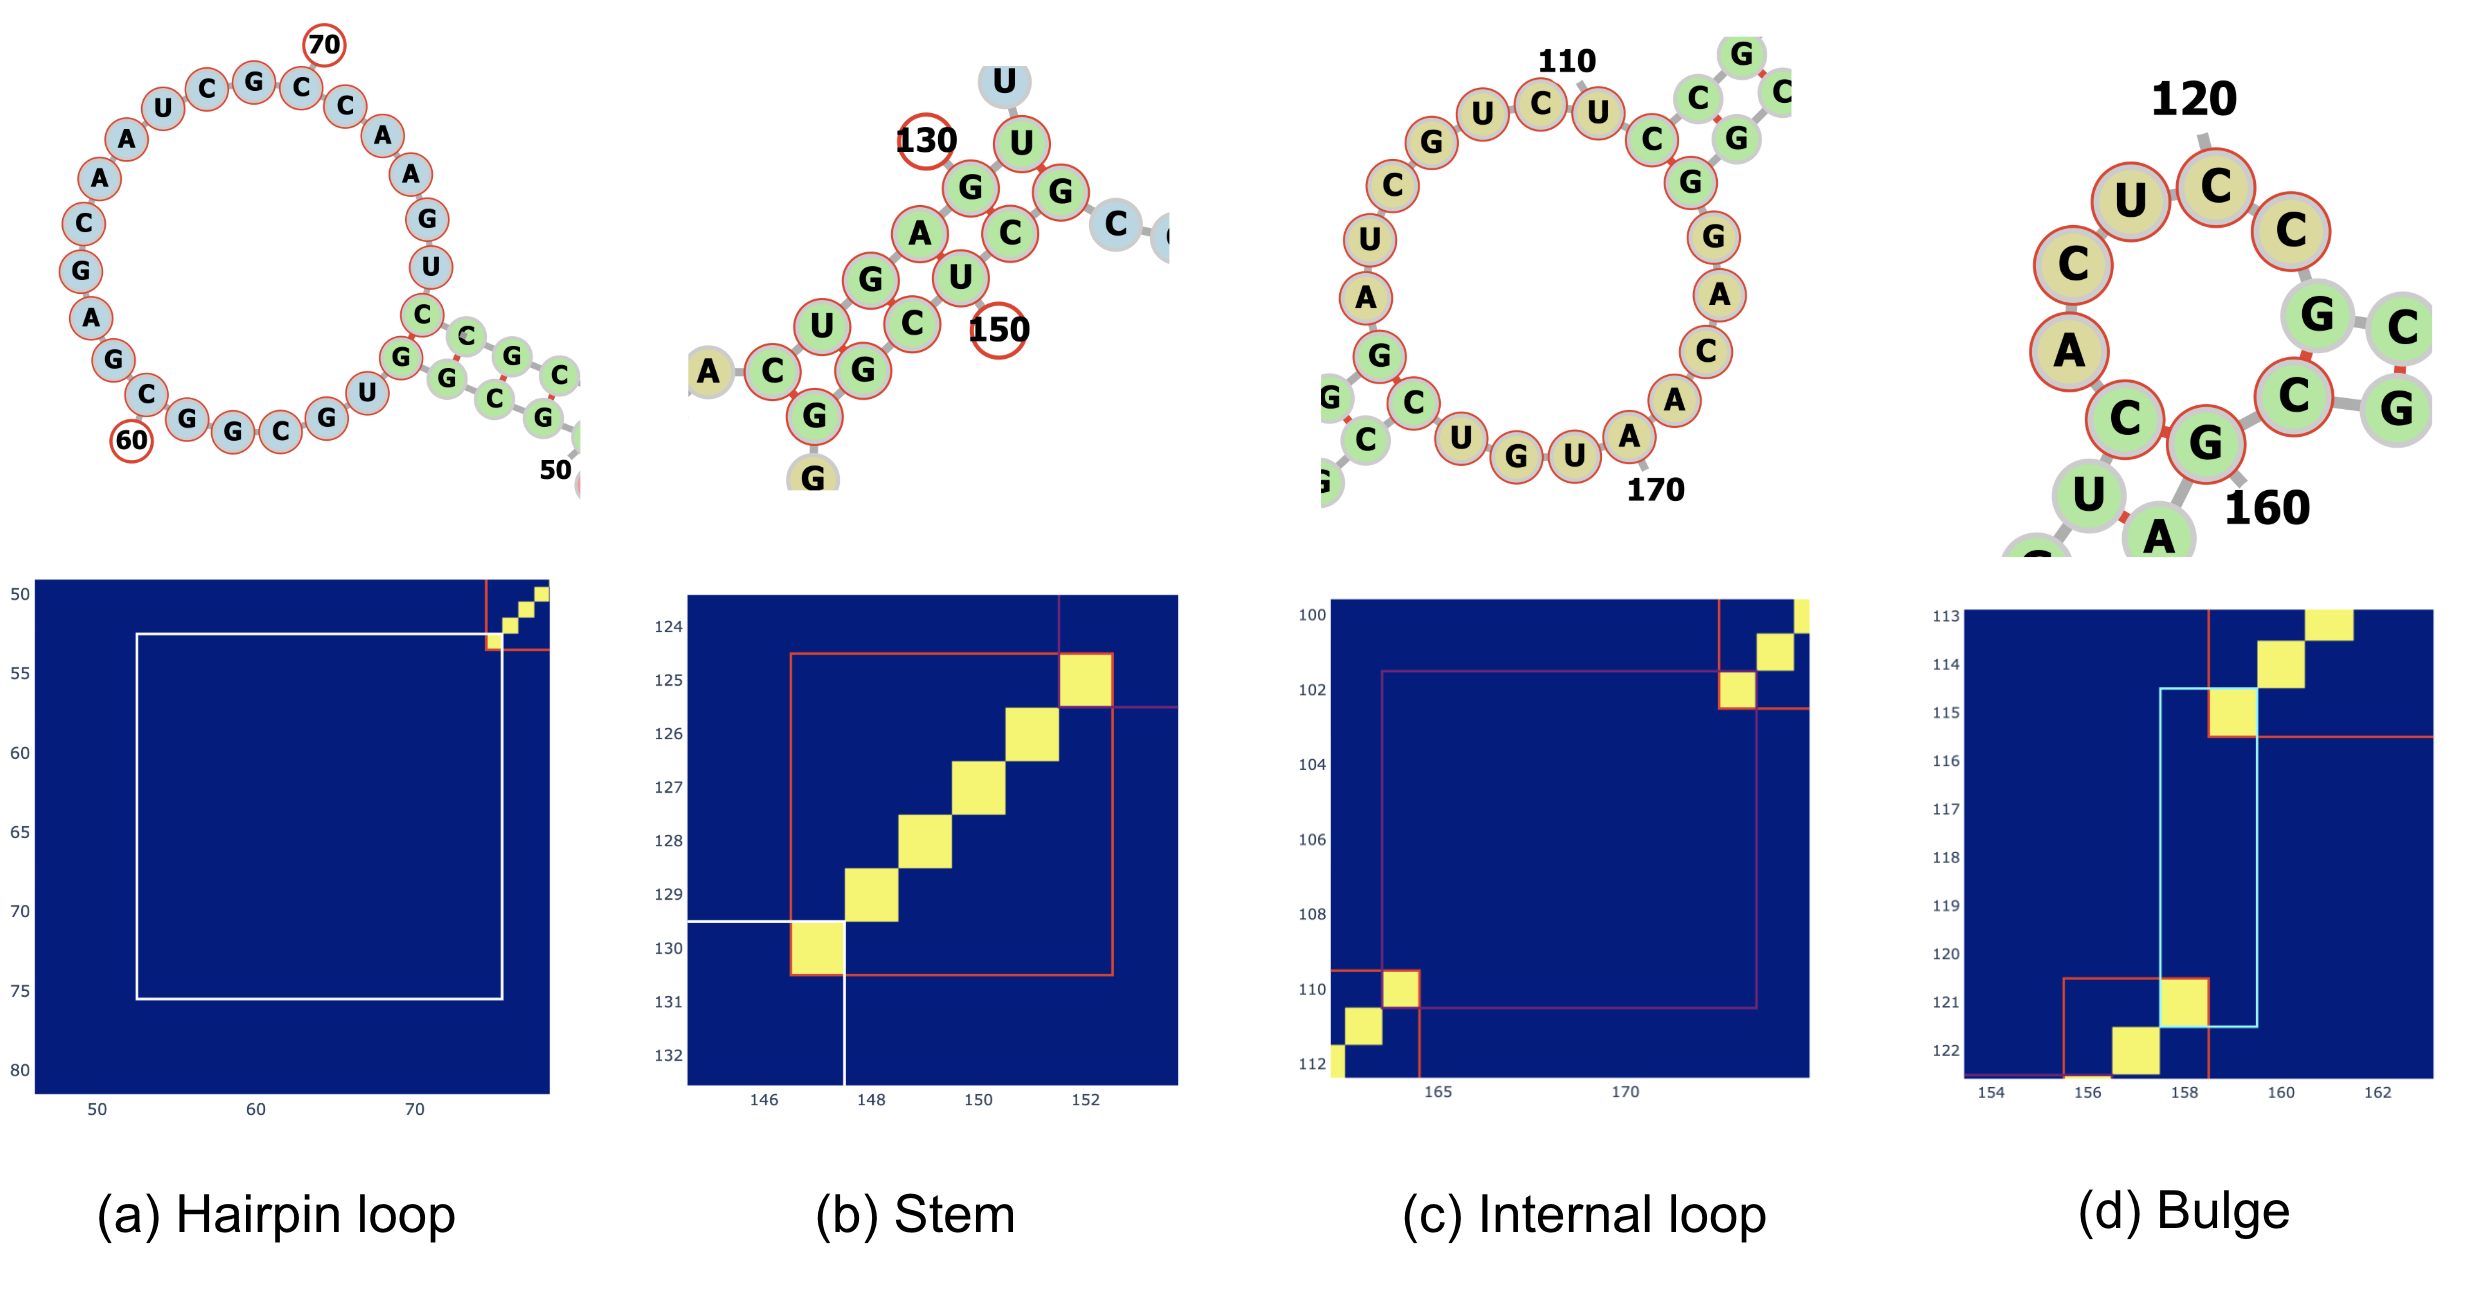
\includegraphics[width=\textwidth]{plot/local_bounding_box_examples.png}
    \caption{TODO}
    \label{fig:local_bounding_box_examples}
    \centering
\end{figure}


To precisely define what constitutes each type of local structure,
we zoom in to each annotated structure in Fig \ref{fig:structural_motif_graph},
and compare it with the corresponding portion zoomed-in on 2D matrix, as shown in
Fig \ref{fig:local_bounding_box_examples}.
We can see that:

\begin{itemize}
    \item hairpin loop: Fig \ref{fig:local_bounding_box_examples}(a),
    square bounding box across the diagonal, all pixels have value $0$ except the top right corner being $1$,
    where the top right pixel corresponds to the
    closing base pair, i.e. the base pair that's 'shared' between the hairpin loop and the stem.
    Note that hairpin loop does not exist in a stand-alone fashion.
    There is always a stem next to it.

    \item stem: Fig \ref{fig:local_bounding_box_examples}(b),
    square bounding box with $1$'s on the off-diagonal and $0$'s elsewhere.


    \item internal loop: Fig \ref{fig:local_bounding_box_examples}(c),
    rectangular (or square) bounding box of all $0$'s except the top right and bottom left corner being $1$,
    where these two pixels correspond to the closing base pairs, one on each side.
    Note that internal loop does not exist in a stand-alone fashion.
    There is always two stems next to it, one on each side.

    \item bulge: Fig \ref{fig:local_bounding_box_examples}(d),
    almost the same as internal loop, except for the bounding box size is constrained
    to be $2xN$ or $Nx2$, since one of the 'side' only has $2$ consecutive base pairs, by definition.
\end{itemize}

One notable fact is that all pixel values inside the bounding box are deterministic given the box type and shape.
This also guarantees that hard constraints are satisfied within each bounding box.

\subsection{Non-local structures}

We're left with $3$ structural motif types that cannot be repsented by a bounding box on 2D matrix.
We will show that non of these structures contribute pixel value of $1$ in the 2D matrix,
and that their existence can be described in an alternative way,
which pinpoint how local structures can be assembled into \textit{valid} global structures.

\begin{figure}[h]
    \centering
    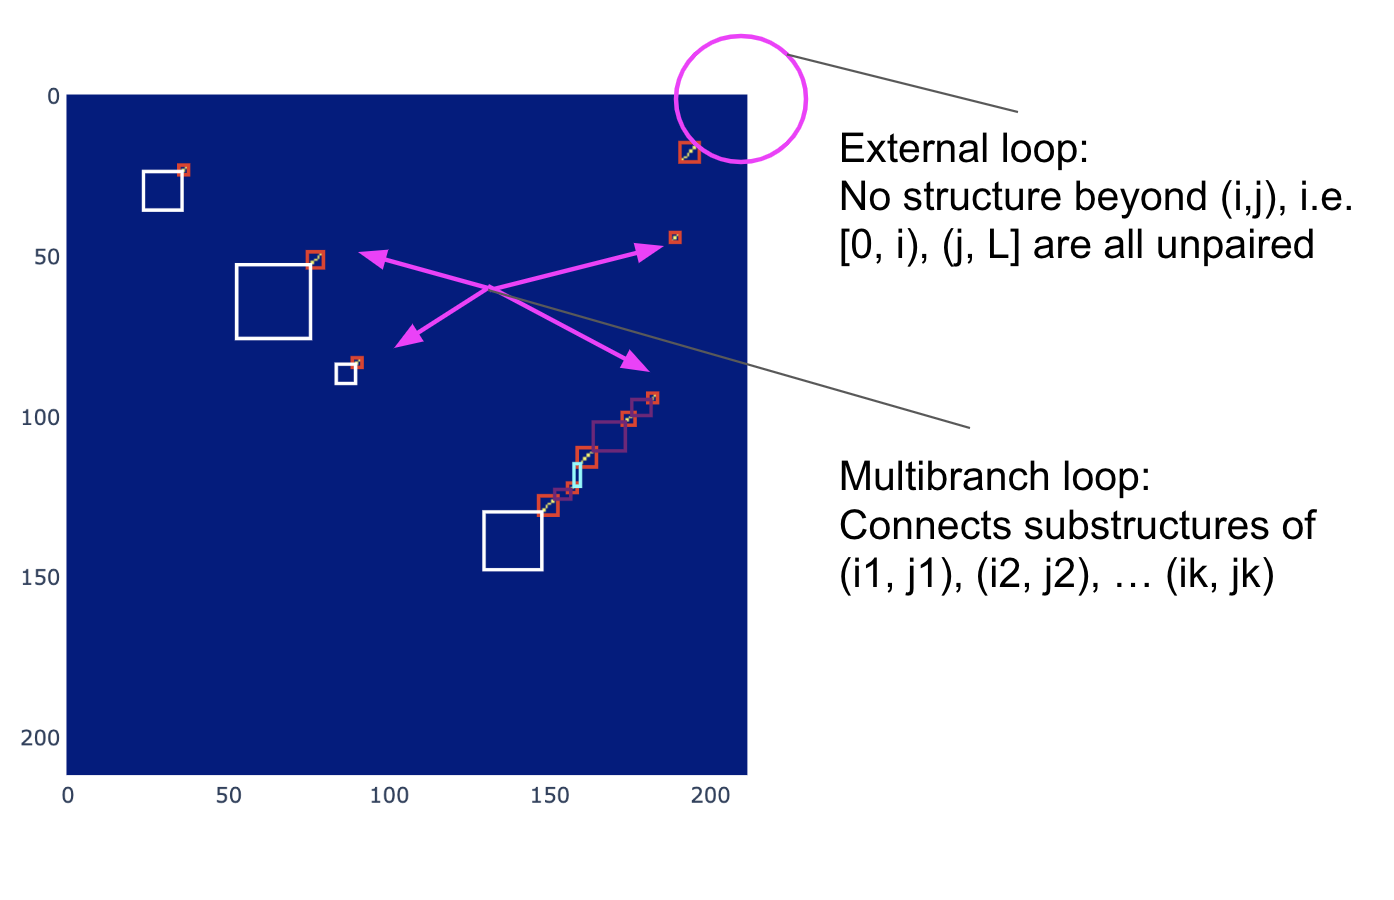
\includegraphics[width=\textwidth]{plot/non_local_structures_2d_matrix.png}
    \caption{TODO}
    \label{fig:non_local_structures_2d_matrix}
    \centering
\end{figure}


\begin{figure}[h]
    \centering
    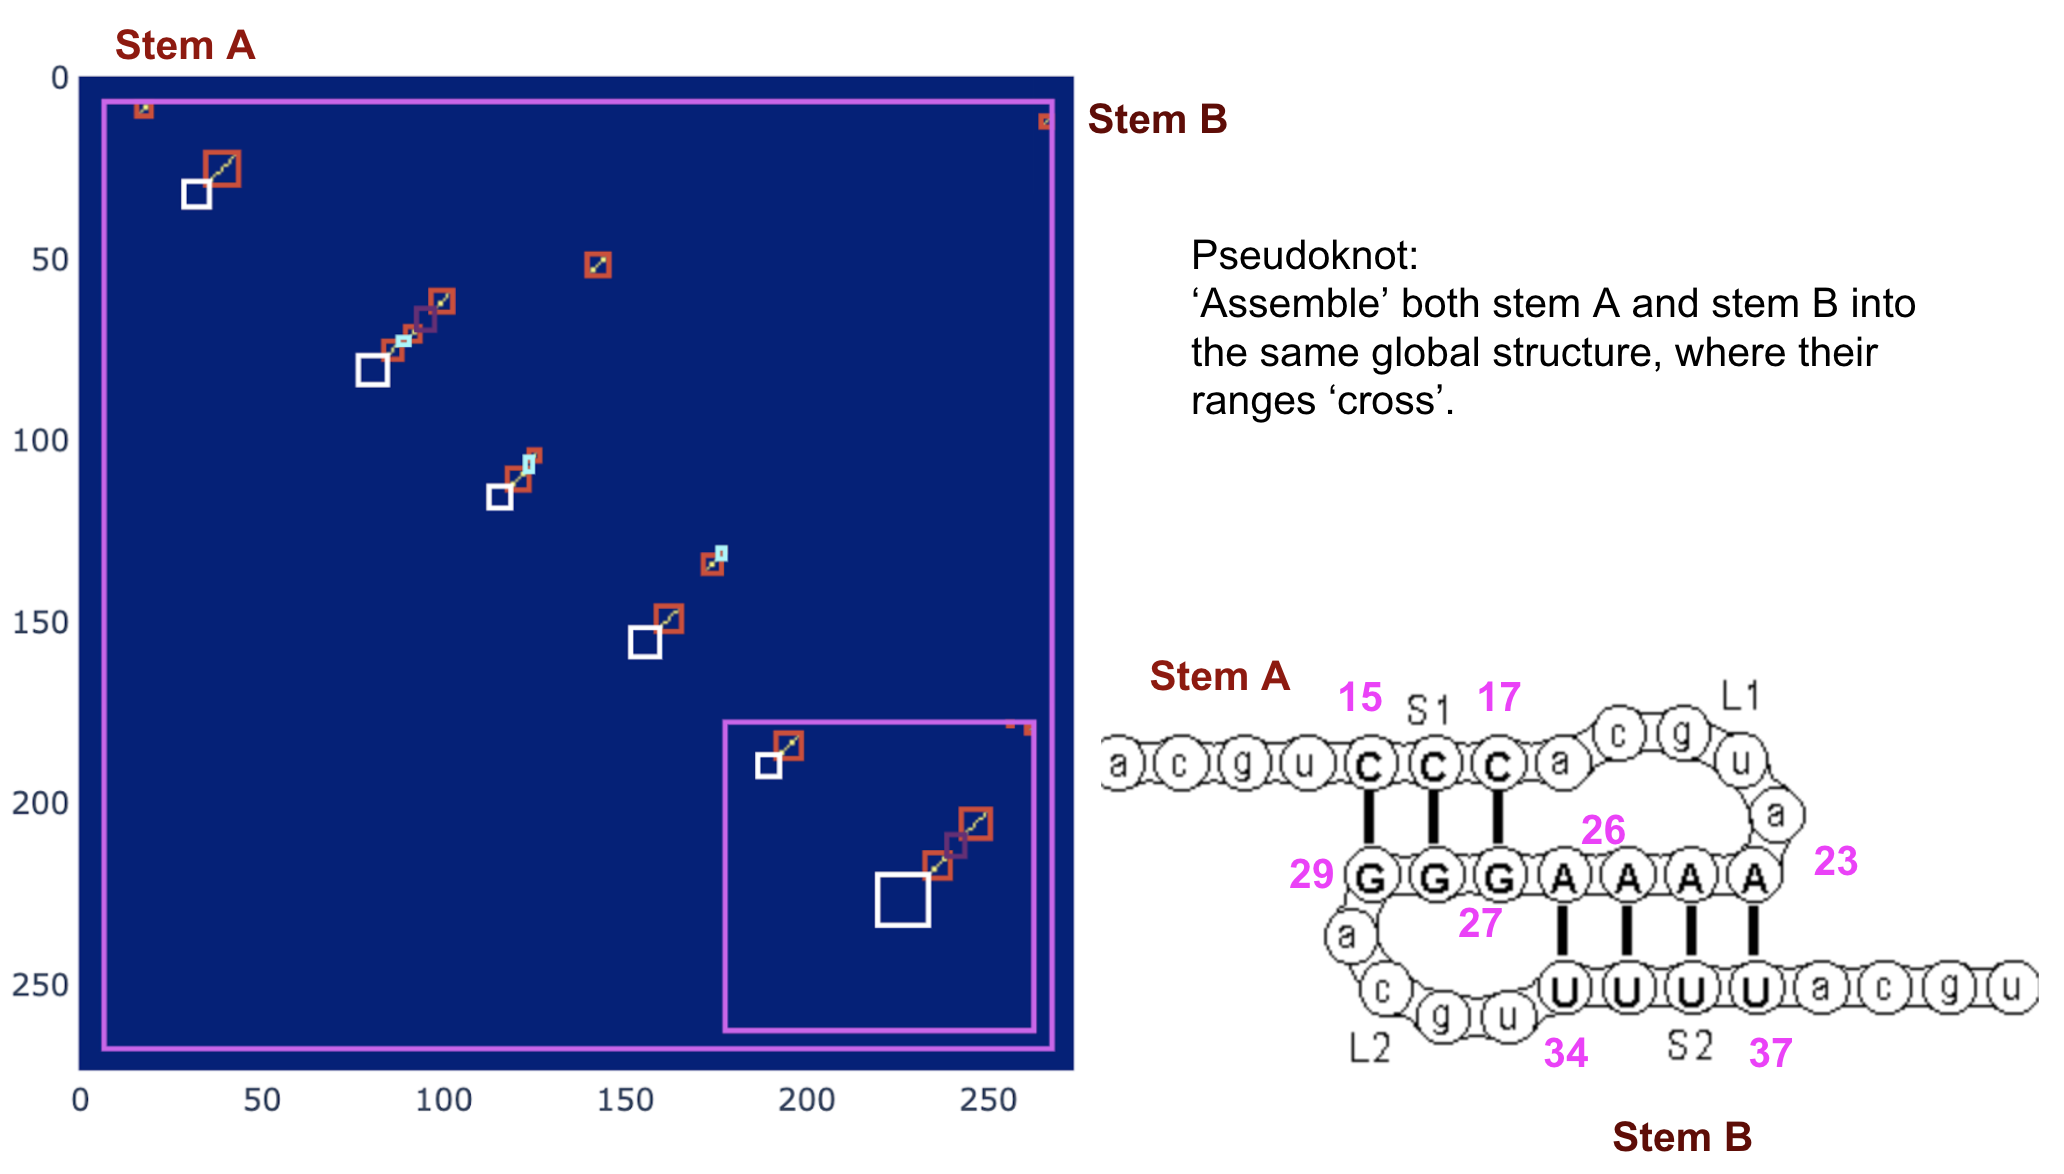
\includegraphics[width=\textwidth]{plot/non_local_structures_pseudoknot.png}
    \caption{TODO}
    \label{fig:non_local_structures_pseudoknot}
    \centering
\end{figure}




\begin{itemize}
    \item external loop: Fig \ref{fig:non_local_structures_2d_matrix},
    the presence of external loop beyond $(i, j)$ indicates that
    bases $0 \dots i$ and $j \dots L$ are all unpaired in the global structure,
    while $i$ and $j$ are paired (not necessarily to each other).
    One might claim that in this particular example it can be fully characterized by a 2D bounding box
    with botton left pixel $(i, j)$ being $1$ since $i$ and $j$ are paired,
    but in practise external loop can also be multi-branch,
    i.e. joining multiple stems, in which case $i$ pairs with some other $k$ and $j$ pair with some other $u$.

    \item multibranch loop: Fig \ref{fig:non_local_structures_2d_matrix},
    the presence of multibranch loop implies that multiple substructures get
    "assembled" into the same global structure, where each substructure is lead
    by a stem whose closing base pair is $(i_k, j_k)$.

    \item pseudoknot: We use a different structure to illustrate pseudoknot
    since the structure we used above does not contain any, see Fig \ref{fig:non_local_structures_pseudoknot}.
    In this example, stem A defines bases $15 \dots 17$ pair with $27 \dots 29$,
    and stem B defines bases $23 \dots 26$ pair with $34 \dots 37$.
    They form a pseudoknot since their ranges cross each other, i.e. non-nested (which is required by most thermodynamic folding).


\end{itemize}



\section{Method}

We propose a 2-stage approach to predict secondary structure from sequence.
In stage 1, we predict all plausible local structures, represented as various types of bounding boxes.
In stage 2, we evaluate all \textit{valid} combinations of local structures from stage 1,
and predict the most likely global structure.
Non-local structure is being modeled implicitly in stage 2 by defining what combinations are valid.

Benefit of such model:

\begin{itemize}
    \item Output is guaranteed to satisfy all hard constraints.
    This is a direct result of the 2-stage approach:
    local structures predicted from stage 1 is parametrized as bounding boxes whose underlying pixels
    satisfy constraints by design.
    Combination of local structure in stage 2 needs to be valid, where validity is precisely defined by hard constraints.

    \item Possibility of predicting sub optimal structure and structure ensemble.
    Since stage 1 predicts all plausible local structures, and stage 2 evaluates the
    likelihood or score of all valid combination, we can predict sub optimal structure,
    and even the entire ensemble.

    \item Support prediction of pseudoknot by design.
    Historically. pseudoknot is difficult to predict since the traditional methods
    were based on recursion defined at a base-pair level,
    thus the nested structure assumption has to be made to result in efficient
    dynamic programming algorithm.
    Our approach evaluates valid combinations of local structure
    (rather than at the base-pair level), whose search space is way smaller than
    evaluating all valid combination of base pairs, so we no longer require the basic components
    (local structures in our case) to be nested, thus enabling pseudoknot prediction.

    \item Can be potentially fine-tuned using probing data.
    Since stage 1 model predicts plausible local structure, and each type of local structure
    implies certain base-pairing or unpairing for the underlying bases,
    we can use probing data to fine-tune the prediction.
    For example, cross-link based RNA probing method detects single and double stranded regions of a RNA,
    and for the double stranded region, although it does not detect the exact base pairing,
    it is possible to infer roughly which region binds to which other region.
    Such information can be incorporated while training the stage 1 model.

\end{itemize}

This report focus on stage 1 model.


\section{Stage 1: Predict local structure}

\subsection{Problem formulation}

Given a input sequence of length $L$,
we would like to predict all plausible local structure bounding boxes in the 2D $L x L$ matrix.
Such problem is well studied in computer vision under the topic of object detection,
from which we got a lot of inspiration.
We notice the following difference compare to object detection in computer vision applications:

\begin{itemize}
    \item In computer vision, the exact pixel location of the bounding box does not matter,
    as long as the bounding box captures the object of interest.
    In our case, since a different pixel correspond to different nucleotides,
    and most of our bounding boxes are small in pixel size, we cannot tolerate even a single pixel shift.

    \item In computer vision, two bounding boxes can overlap
    if the underlying objects overlap on the image. In our case, for a set of bounding boxes to
    be part of the same global structure, they cannot overlap (except for corner pixels),
    since the location and size of each bounding box fully parameterize the pixel values it encapsulates.

    \item In computer vision training dataset, the bounding box annotations can be considered
    accurate enough in the sense that most positive examples are being annotated with bounding boxes,
    and regions without bounding boxes typically have no objects of interest (unless it was wrongly annotated).
    In contrast, a typical RNA SS training dataset consists of sequence-structure pairs,
    where there is *one* structure per sequence. Such structure typically represent the \textit{most likely}
    global structure. There can be some other sub optimal global structure that are \textit{less likely globally},
    but their underlying local structure could still be plausible.
    This means that if we parse this particular global structure into local structure components and use them for training,
    these local structures can be considered positive examples without any problem,
    but in regions where no local structure is present where we consider all being negative examples there could potentially be false negatives.
\end{itemize}

With the above in mind, we propose the following setup for model training.
For each pixel in the output $L x L$ matrix, we would like to assign it to some bounding box(es),
and we would also want the location and size of the bounding boxes to be encoded with pixel-precision,
so that we can try to predict the presence, location and size of the bounding boxes.



Most of the time, each pixel can be uniquely assigned to one bounding box.
In the case of closing pair of a loop, it's assigned to both the stem and the loop,
for example, see the pixel where two bounding boxes overlap in Fig \ref{fig:local_bounding_box_examples}.
In the rare case where the stem is of length $1$, and the stem has $2$ loops, one on each side,
the pixel is assigned to $2$ loops. We'll ignore this rare case for now and work on it as part of future improvement.
Furthermore, we notice the fact that the bounding box for bulge can can be considered a special case of internal loop,
where the height or width is constrained to be $2$, so for now we combine these two into one category and we will refer to
it as \textit{internal loop}.
Thus, it can be observed that each pixel can be assigned to:

\begin{itemize}
    \item 0 or 1 stem box
    \item 0 or 1 internal loop box
    \item 0 or 1 hairpin loop
\end{itemize}

From the above, we can easily see that for each pixel we need at most 3 bounding boxes,
each with its unique type (stem/internal loop/hairpin loop),
and each bounding box can be on/off independent of the others.
Using the above formulation, we only need to predict the on/off of each box (sigmoid),
without the need to predict its type (avoid problem of multiple box permutation in computer vision).

For each pixel, we set the corresponding bounding box to be \textbf{on} if the pixel is within the bounding box.
To encode the location od bounding box (w.r.t. the pixel),
we use the top right corner odf bounding box as the reference point,
and calculate the distance of the current pixel to the reference,
both horizontally and vertically.
The idea is to predict it using a softmax over finite classes so we can predict the pixel-precision location.
Horizontal distance (y/columns) is always $<= 0$: $ 0, -1, \dots, -9, -10, -10_beyond$,
and vertical distance (x/rows) is always $>= 0$: $0, 1, \dots, 9, 10, 10_beyond$,
i.e. we assign one class for each integer distance until some distance away ($10$ in the above example).


To encode the size, we use different number of softmax, depending on the box type.
For stem there is one softmax over $1, \dots, 9, 10, 10_beyond$, since it's square shaped.
For internal loop we have two softmax over $1, \dots, 9, 10, 10_beyond$, one for height one for width.
For hairpin loop there is one softmax over $1, \dots, 9, 10, 10_beyond$, since it's square shaped.
Note that for both location and size, the integer cutoff of $10$ is an arbitrary choice for now,
and we'll look into how to support larger ones in future work.

\begin{figure}[h]
    \centering
    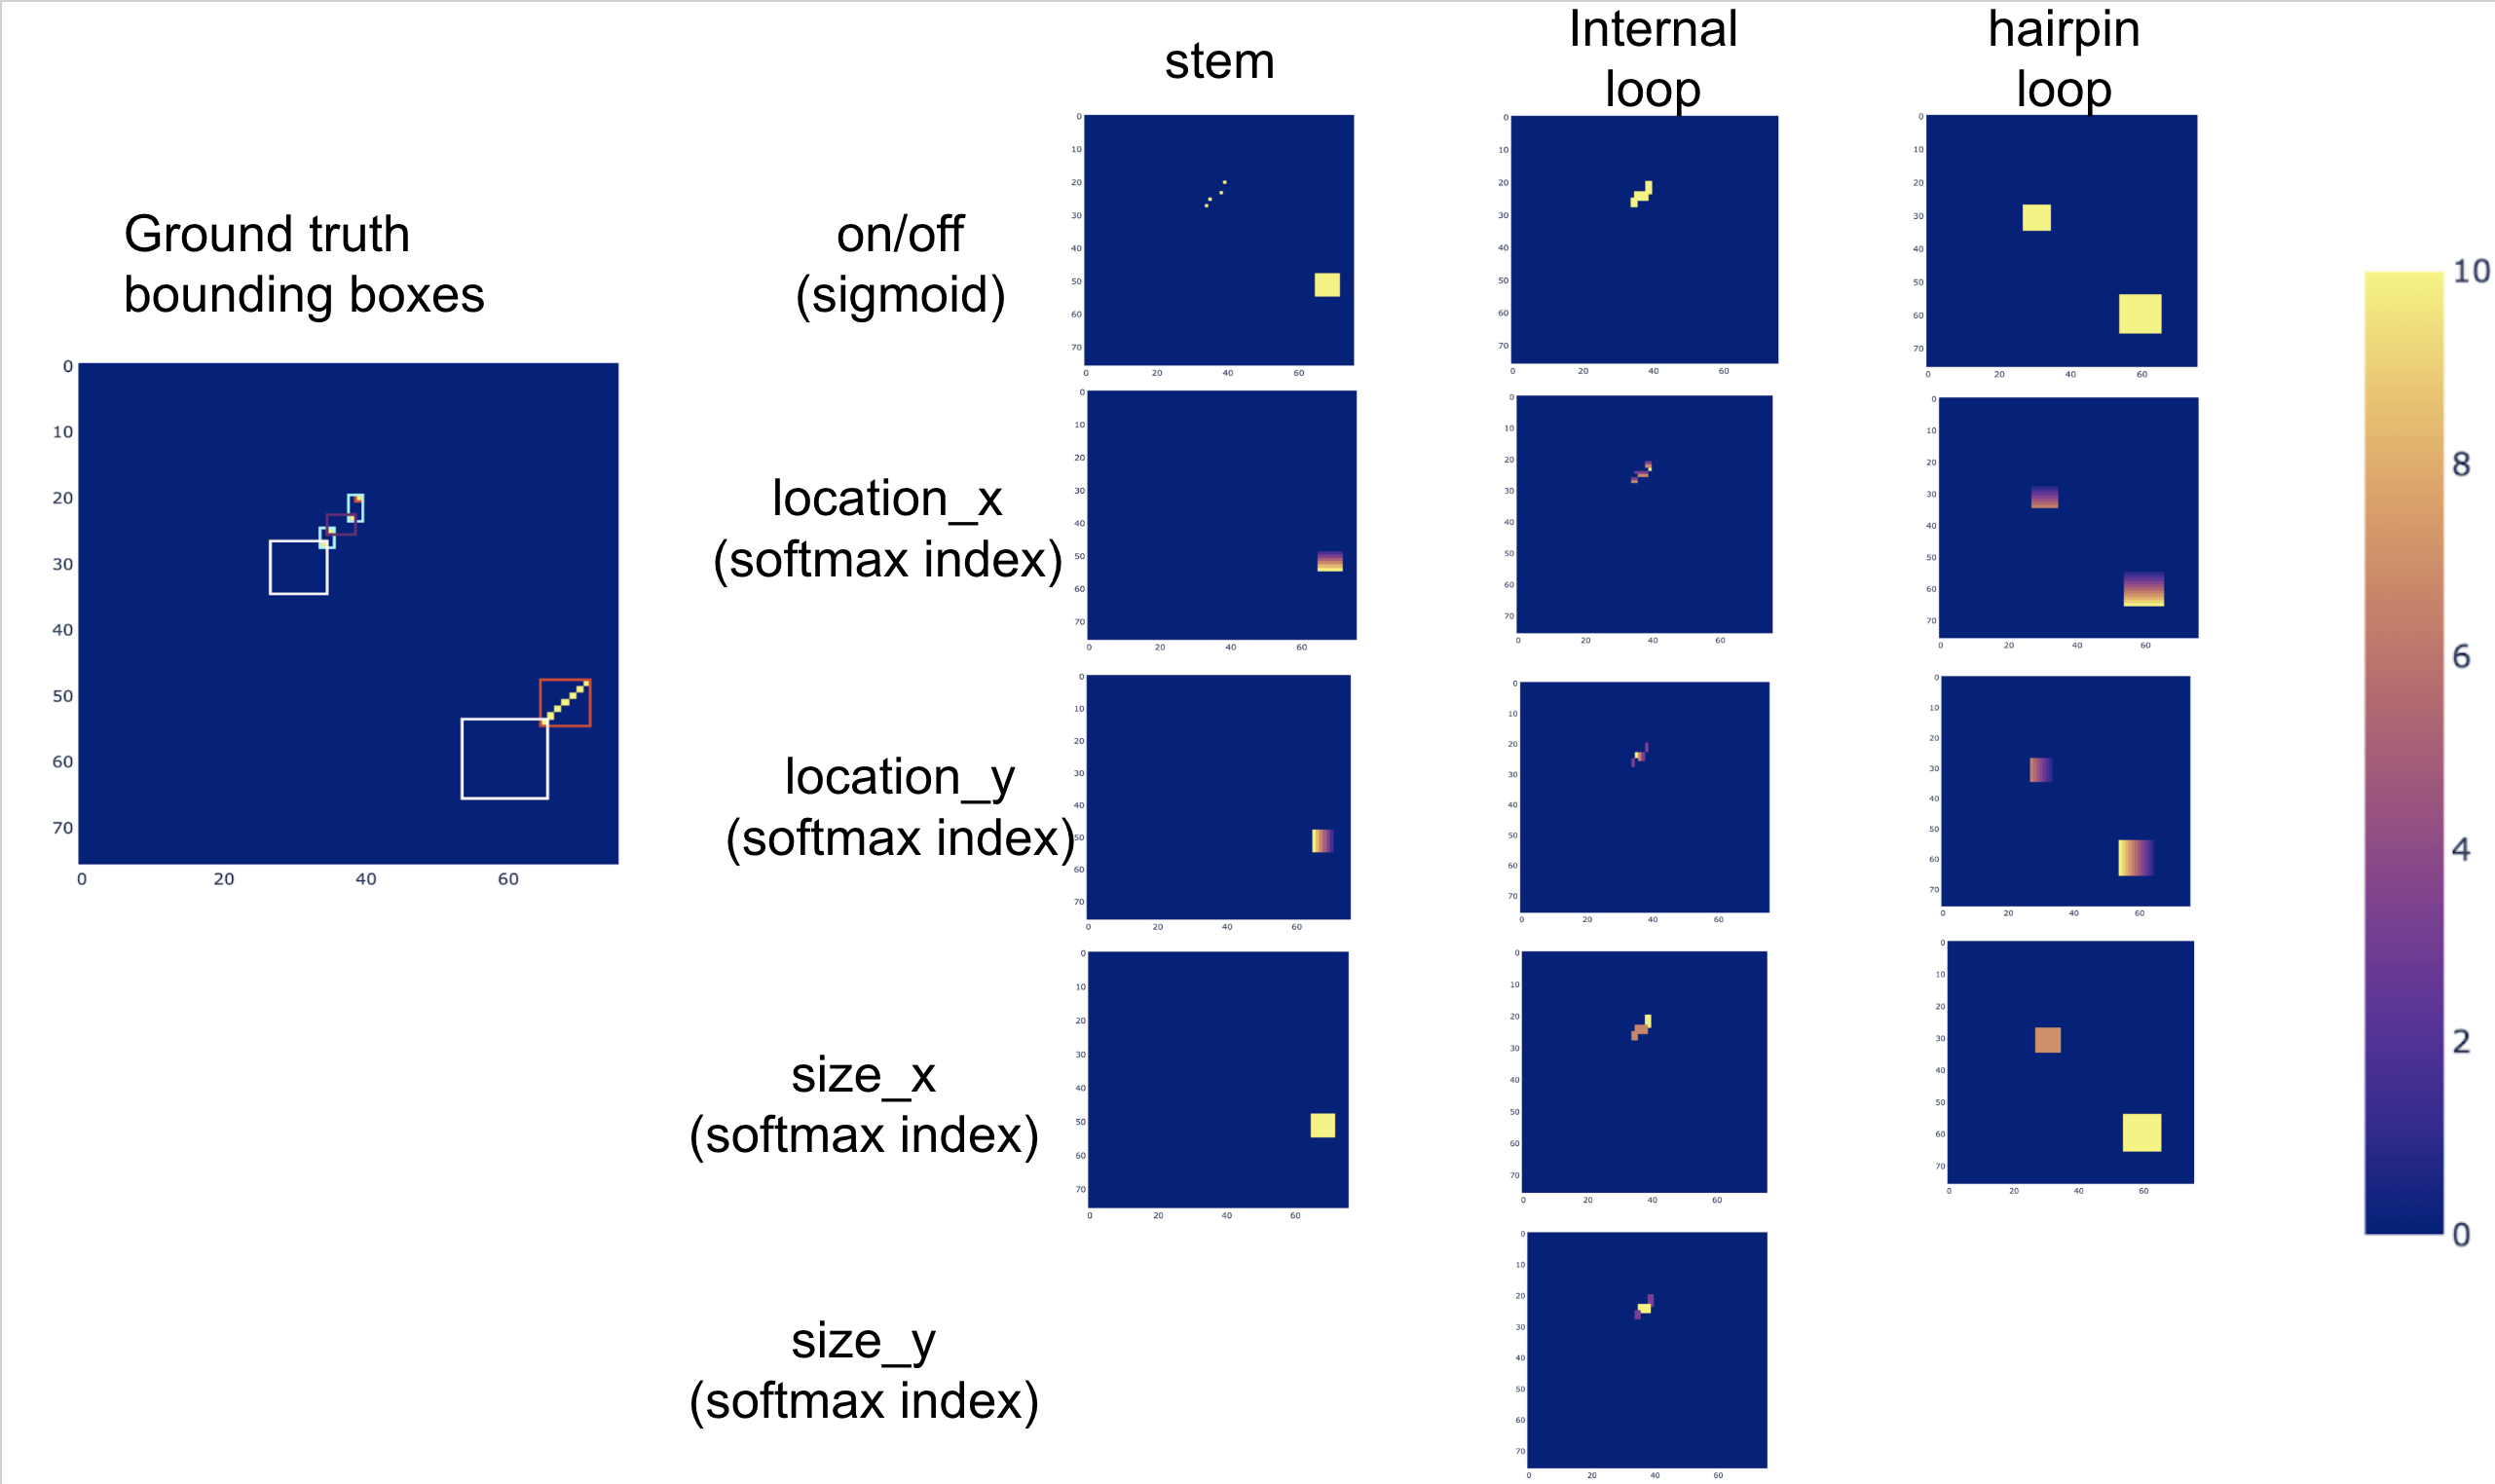
\includegraphics[width=\textwidth]{plot/training_pixel_targets.png}
    \caption{TODO}
    \label{fig:training_pixel_targets}
    \centering
\end{figure}

In summary, each pixel in the training dataset has $13$ targets,
as demonstrated in Fig \ref{fig:training_pixel_targets}:

\begin{itemize}
%    \item stem\_on
    \item \textit{stem\_on}: stem on off probability, sigmoid
    \item \textit{stem\_location\_x}: vertical distance between stem bounding box reference and current pixel, softmax with 12 classes
    \item \textit{stem\_location\_y}: horizontal distance between stem bounding box reference and current pixel, softmax with 12 classes
    \item \textit{stem\_size}: stem bounding box size, softmax with 11 classes

    \item \textit{iloop\_on}: internal loop on\/off probability, sigmoid
    \item \textit{iloop\_location\_x}: vertical distance between internal loop bounding box reference and current pixel, softmax with 12 classes
    \item \textit{iloop\_location\_y}: horizontal distance between internal loop bounding box reference and current pixel, softmax with 12 classes
    \item \textit{iloop\_size\_x}: internal loop bounding box height, softmax with 11 classes
    \item \textit{iloop\_size\_y}: internal loop bounding box width, softmax with 11 classes

    \item \textit{hloop\_on}: hairpin loop on\/off probability, sigmoid
    \item \textit{hloop\_location\_x}: vertical distance between hairpin loop bounding box reference and current pixel, softmax with 12 classes
    \item \textit{hloop\_location\_y}: horizontal distance between hairpin loop bounding box reference and current pixel, softmax with 12 classes
    \item \textit{hloop\_size}: hairpin loop bounding box size, softmax with 11 classes
\end{itemize}



\subsection{Model and training}

We use 2D conv net to predict the bounding boxes for all pixels in parallel.
For a sequence $s$ of size $L$, the input $x$ is of size $L x L x 8$, where $x[i, j, :]$
in the concatenation of one-hot encoding of nucleotide $s[i]$ and $s[j]$.
There are $13$ targets (a combination of sigmoid and softmax) for each pixel,
as indicated in the previous section.


We use a synthetic dataset to train the bounding box model (we're reserving the 'real' dataset for stage 2 model to predict global structure).
Specifically, we generate random sequences of various length up to $200$, and use RNAfold to generate the
minimum free energy structure and split into into local structures and annotate the corresponding bounding boxes.
For each pixel, we check whether it's within a bounding box (for each of the $3$ types),
if so we calculate the location of bounding box w.r.t. the pixel and assign the corresponding target values for the sigmoid and softmax.

For pixels whose bounding box is set to off, the location and size softmax target losses are being masked out,
since we do not have a target value for those and we do not care about the model prediction.
In addition, to account for the fact that training dataset contains many potential false negatives
from the perspective of local structure bounding boxes
(i.e. pixels that do not belong to a bounding box in the particular example, but has a plausible local structure nearby, see Section ???),
we re-weight losses on pixels outside the bounding boxes by a factor of $0.1$ (hard-coded for now, can be treated as hyperparameter).



\subsection{Inference} \label{sec:inference}

At inference time, each pixel can predict up to $3$ bounding boxes, one for each type.
In this section we describe how to predict the stem bounding box, and the other two type are done in a similar way.
For each pixel $(i, j)$, we do the following:

\begin{enumerate}
    \item Apply a threshold on sigmoid output \textit{stem\_on} to determine whether to compute bounding box for that pixel.
    A typical threshold is $0.5$, but a different one can be used considering training data class imbalance,
    as well as loss re-weighting.
    In general, a lower threshold results in more bounding boxes (more false positives and less false negatives),
    which might be desirable to feed as input to stage 2 model.
    \item Compute the maximum likelihood bounding box location and size.
    We maximize probabilities of \textit{stem\_location\_x}, \textit{stem\_location\_y} and \textit{stem\_size},
    by taking the argmax index of each softmax.
    Let the indices be \textit{idx\_x}, \textit{idx\_y}, \textit{idx\_siz}, respectively.
    The location of the predicted bounding box reference point (top right corner) is:

    \begin{equation}
        \begin{align}
            i\_ref = i - idx\_x \\
            j\_ref = j + idx\_y
        \end{align}
    \end{equation}

    and size of bounding box ($+1$ since idx 0 corresponds to size 1):

    \begin{equation}
        size = idx\_size + 1
    \end{equation}

    Note the above does not produce accurate result for bounding box location and size beyond the softmax length (to be worked on in the future).

    \item We can also compute the probability of this bounding box,
    by multiplying the sigmoid probability and 3 softmax probability corresponding to the argmax index:

    \begin{equation}
        p\_box = stem\_on * stem\_location\_x[idx\_x] * stem\_location\_y[idx\_y] * stem\_size[idx\_size]
    \end{equation}

\end{enumerate}

\begin{figure}[h]
    \centering
    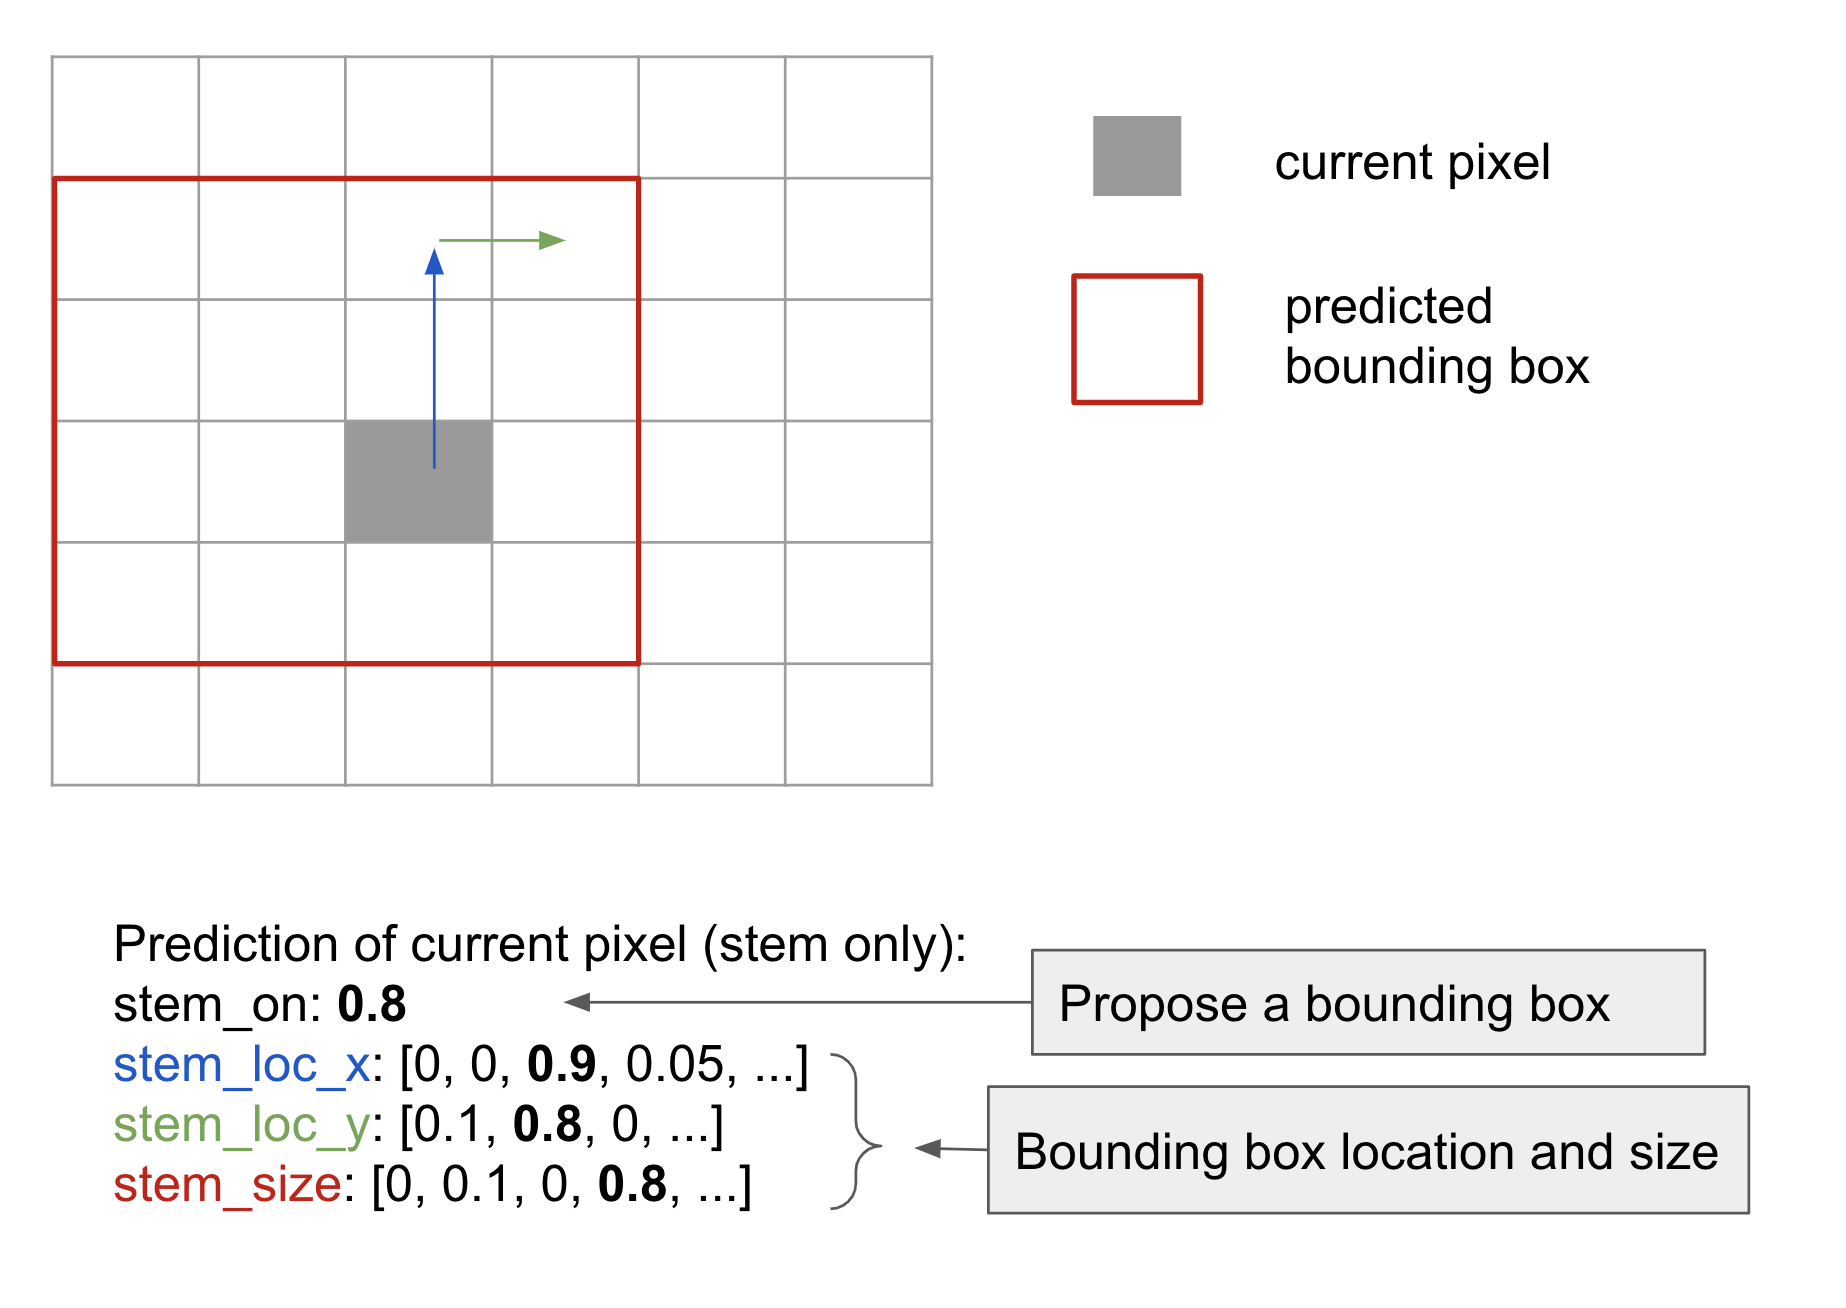
\includegraphics[width=\textwidth]{plot/inference_bb_prediction.png}
    \caption{TODO}
    \label{fig:inference_bb_prediction}
    \centering
\end{figure}


See Fig \ref{fig:inference_bb_prediction} for an example.


\subsection{Result}

Results presented in this section are from the following model:

\begin{itemize}
    \item $7$ 2D conv layers with Relu activation and batch norm
    \item shared hidden layer with $50$ units
    \item each output has its own hidden layer with $20$ units
    \item sigmoid or softmax activation depend on output type
    \item Adam optimizer with learning rate $0.0001$
    \item model trained for $20$ epoches
    \item Dataset of $500,000$ random sequences, $80\%$ used for training and $20\%$ for validation
\end{itemize}

We compute the following performance metrics, for each type of bounding box:

\begin{enumerate}
    \item Sensitivity for identical bounding box:
    given a ground truth bounding box, what's the probability that at least one predicted bounding box is identical.
    \item Sensitivity for overlapping (including identical) bounding box:
    given a ground truth bounding box, what's the probability that at least one predicted bounding box overlaps it.

    \item Pixel specificity:
    for all pixels that overlap predicted bounding box(es), what's the probability it also overlaps a ground truth bounding box.
\end{enumerate}


For each example in the validation set, we compute the above metrics for all bounding box types,
and plot the distribution of these metrics across all examples, as shown in Fig \ref{fig:performance_metrics}.
We can see that for most examples in the validation set the ground truth bounding box can be perfectly reconstructed,
as indicated by high sensitivity for identical bounding box.
Further more, if we relax the reconstruction criteria to be overlapping instead of identical,
sensitivity gets close to $100\%$.
On the other hand, specificity is much lower overall,
which is expected due to false negatives in the training dataset.
We want to also point out that at this stage a high sensitivity and lower specificity is desired,
since in stage 2 where we combine local structures into global structure, many of the proposed bounding boxes
would probably be left out due to their incompatibility with other bounding boxes.


\begin{figure}[h]
    \centering
    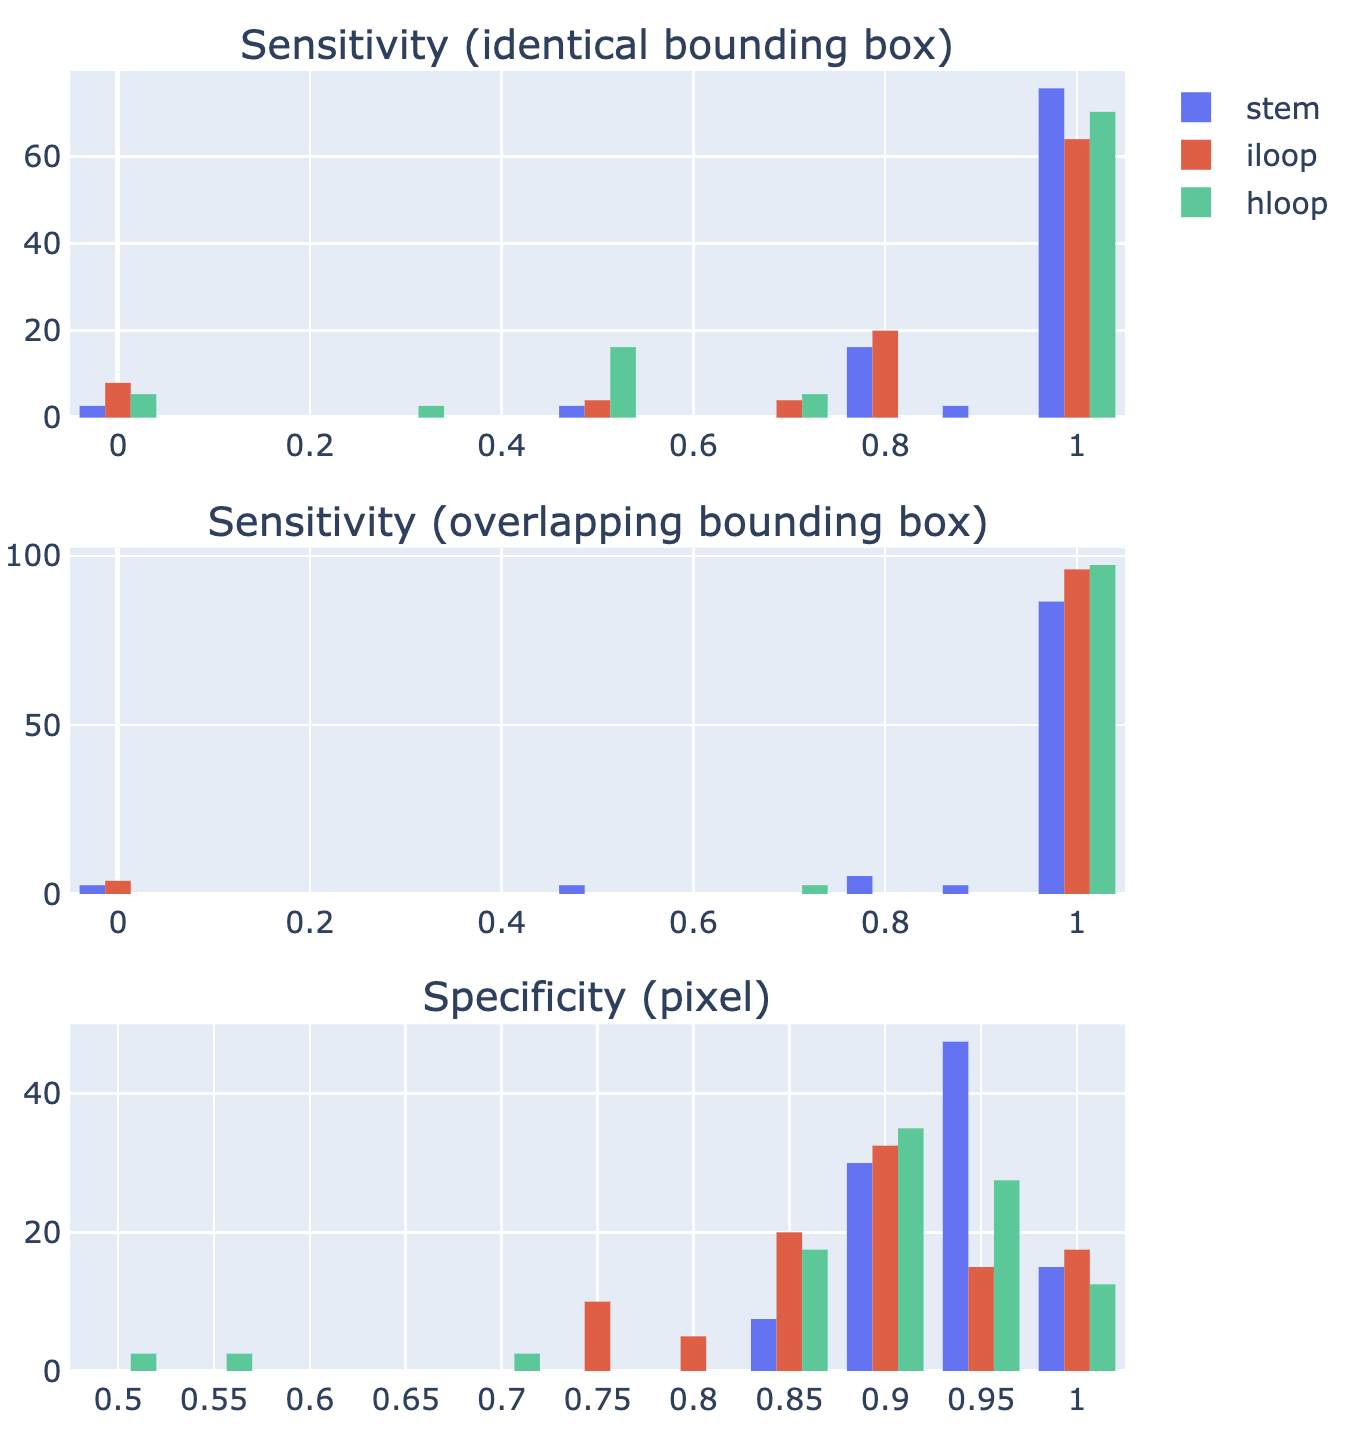
\includegraphics[width=0.8\textwidth]{plot/performance_metrics.png}
    \caption{TODO}
    \label{fig:performance_metrics}
    \centering
\end{figure}






\subsection{Visualize bounding box prediction}

To get a concrete idea on how well the model reconstructs the local structure bounding boxes,
we visualize the predicted bounding boxes for one example in the validation set, as shown in Fig \ref{fig:visualize_bb_prediction}.
Here we've applied a cutoff $0.2$ to all sigmoid units to find all pixels where bounding box(es) should be computed.
Then for each such pixel, we calculate the location and size of bounding box,
and draw the bounding box with opacity set to the probability of the box.
Bounding box proposed from neighbouring pixels can overlap partially or entirely.
Visually, a \textit{darker} bounding box is a more confident one,
since it corresponds to a high probability box and/or identical proposals from multiple pixels.
Predicted bounding boxes in red, while Solid yellow color blocks are ground truth.

\begin{figure}[h]
    \centering
    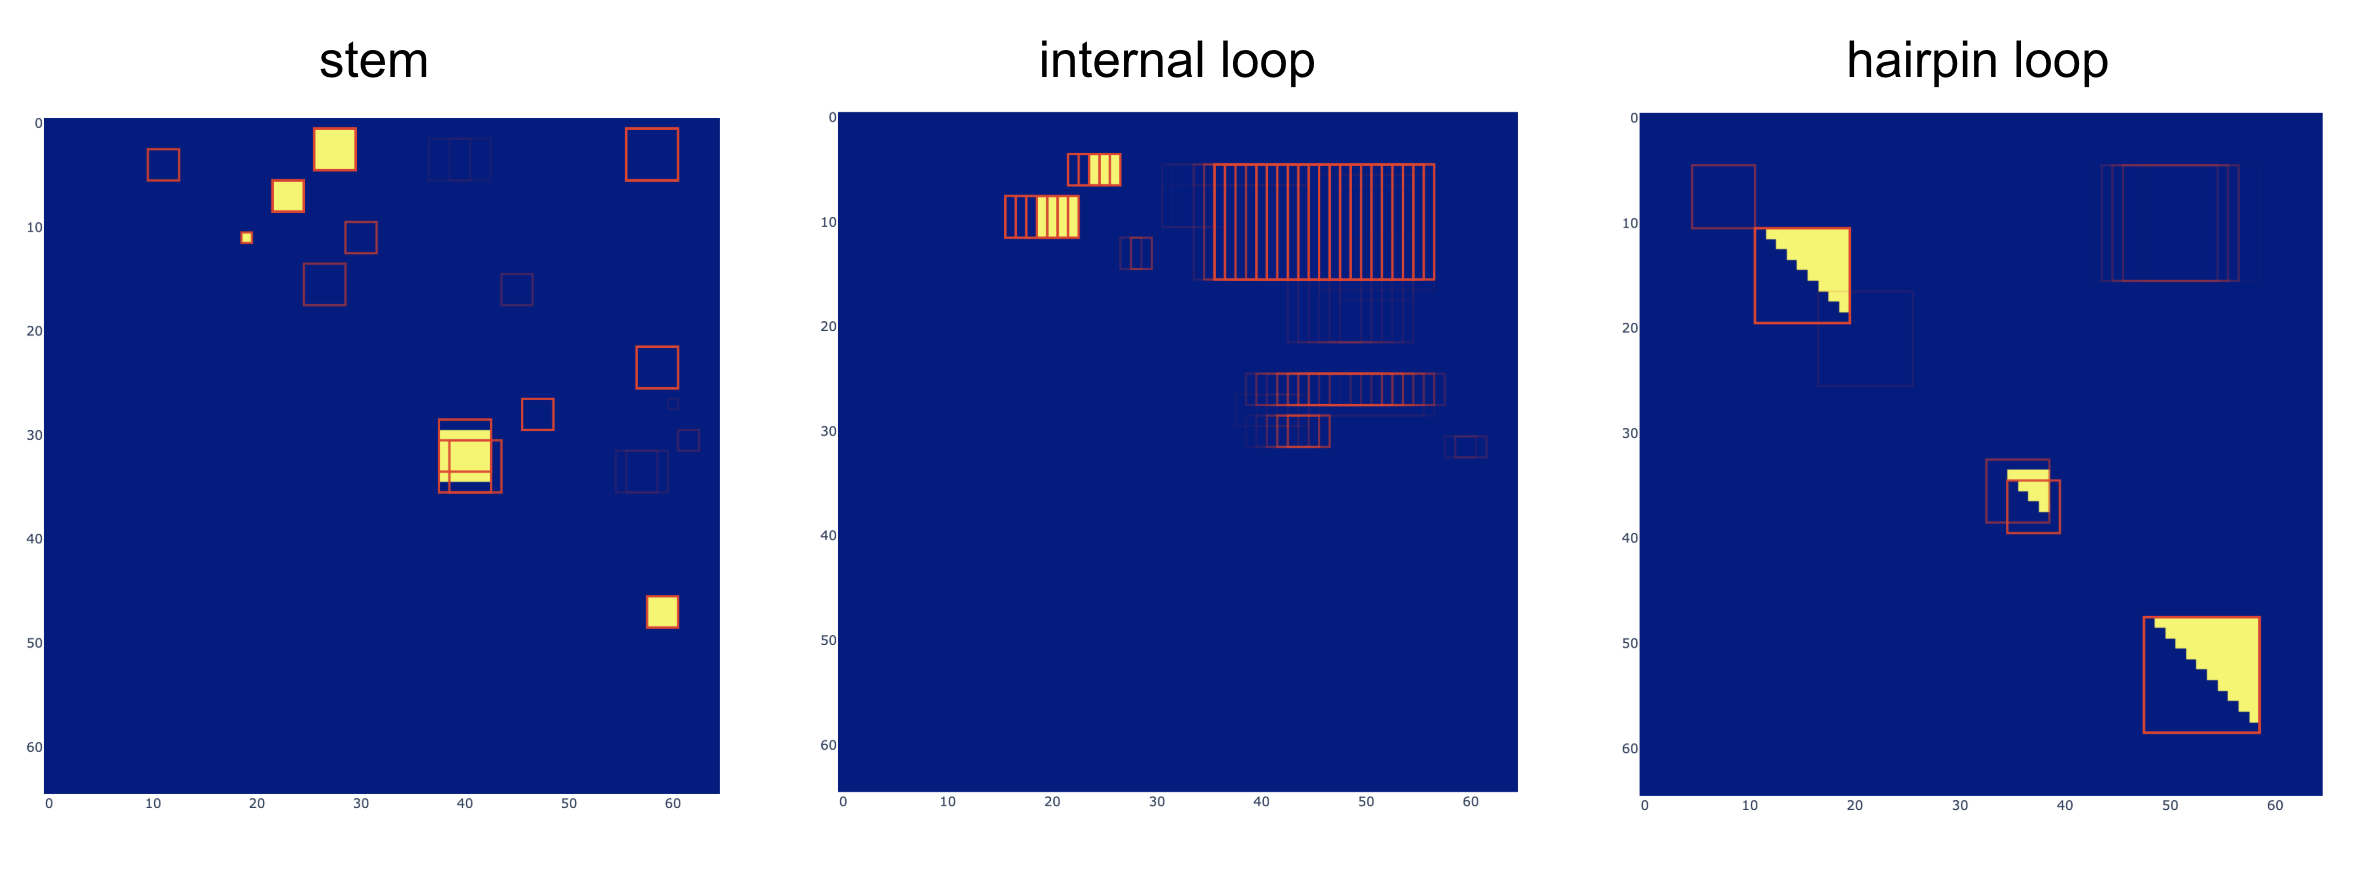
\includegraphics[width=\textwidth]{plot/visualize_bb_prediction.png}
    \caption{TODO}
    \label{fig:visualize_bb_prediction}
    \centering
\end{figure}



\section{Ideas for Stage 2: global structure assembly}


\section{Future work}

satisfy constraints,
all possible 2D binary matrix -> huge space, majority does not satisfy biology constraints.
bounding box: parameterized by a few parameters,
pixel value implied given parameterized, satisfy (local) constraints.



todo larger sequence efficient

conv filter redundancy

incompatibility of softmax

%\bibliographystyle{unsrt}
%\bibliography{report}


\end{document}
